\documentclass{standalone}

\usepackage{tikz,pgf}
\usepackage[utf8]{inputenc}
\usepackage[colorlinks=true, allcolors=blue]{hyperref}
\usetikzlibrary{positioning, arrows.meta, fit, shapes}
\begin{document}


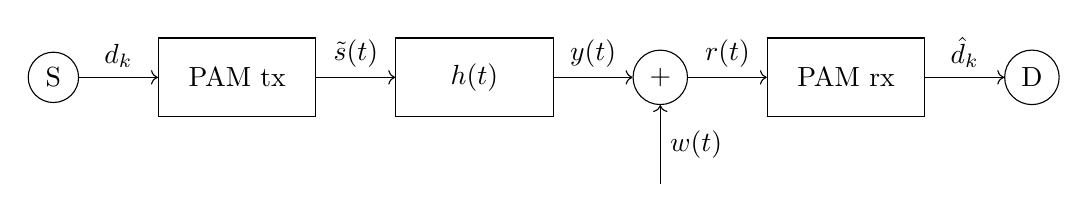
\begin{tikzpicture}[
            block/.style={rectangle, draw, minimum height=1cm, minimum width=2cm},
            node distance=1cm,
            auto
        ]
        \node[draw, circle] (source)  {S};
        \node[block, right= of source] (interpolatore) {PAM tx};
        \node[left=of interpolatore] (tmp) {};
        \node[block, right= of interpolatore] (chan) {$h(t)$};

        \node[draw, circle, right= of chan] (plus)  {\(+\)};
        \node[below=of plus, inner sep=0pt, minimum size=0pt] (n) {};
        \node[block, right=of plus] (sampler) {PAM rx};
        \node[circle, draw, right=of sampler] (dest) {D};
        
        \draw[->] (source) -- (interpolatore) node[midway,above] {$d_k$};
        \draw[->] (interpolatore) -- (chan) node[midway,above] {$\tilde{s}(t)$};
        \draw[->] (chan) -- (plus) node[midway,above] {$y(t)$};
        \draw[->] (plus) -- (sampler) node[midway,above] {$r(t)$};
        \draw[->] (n) -- (plus) node[midway, right] {$w(t)$};
        \draw[->] (sampler) -- (dest) node[midway,above] {$\hat{d}_k$};
    \end{tikzpicture}



\end{document}
